\section{Implementación}
\noindent Las tareas realizadas pueden clasificarse en tareas de visión por computador y tareas de control. En este apartado se explicará cada una de ellas, incluyendo todos los programas realizados a lo largo del proyecto. \\

\noindent Los tópicos de ROS realizan una tarea importante en este trabajo, ya que gracias a ellos podemos escribir códigos en distintos lenguajes de programación, en este caso, la visión en C++ y el control en Python, y compartir información entre ellos. A continuación se explica cada una de estas tareas. \\

\textbf{baxter\_img.cpp} Este código escrito en lenguaje C++ es el encargado del procesamiento de imágenes utilizando OpenCV y de enviar la posición del punto medio entre los dos clústers al tópico \textit{/classification}.\\

\textbf{pick\_and\_place.py} Este programa se subscribe al tópico \textit{/detected\_objects} para obtener la posición de los objetos y construir una torre con ellos. \\

\textbf{classif.py} Este archivo en Python se subscribe al tópico \textit{/classification} y realiza una clasificación de los objetos situados en la mesa. \\

\textbf{dyn\_classif.py} Este otro programa también escrito en Python se subscribe al tópico \textit{/classification} para realizar una clasificación en entorno dinámico con una paleta como herramienta. \\

\textbf{dyn\_wedge.py} Este último programa en Python obtiene el punto medio a través del tópico \textit{/classification} y realiza una clasificación en entorno dinámico con una cuña como herramienta.\\

\textbf{archivo.launch} Estos archivos son los encargados de inicializar el nodo de MoveIt! y RViz, la cámara del brazo derecho de Baxter y los programas de visión y control de cada caso definido anteriormente. \\ 

\textbf{CMakeLists.txt} Archivo que incluye los paquetes, dependencias y librerías que requiere el proyecto. \\

\textbf{package.xml} Define las dependencias de compilación y ejecución que requiere el proyecto además de definir algunas variables como el nombre, la versión o la licencia. \\

\subsection{Esquema general del escenario}
\noindent En este apartado se muestran los componentes utilizados en el escenario y las conexiones que se establecen entre ellos. \\

\begin{itemize}
	\item Objetos a clasificar. Se utilizarán varios objetos de distinto tamaño y color. Además se realizarán tests utilizando mayor o menor número de piezas. \\
	\item Cinta transportadora. Es la mesa sobre la que se posicionan los objetos. Se utilizará tanto en entorno dinámico como en estático. Para realizar la segmentación en entorno dinámico, se utilizarán las primeras velocidades de la cinta, que se pueden regular mediante la rueda de la que dispone la cinta. \\
	\item Baxter. Se utilizará el brazo robótico derecho para el control y la cámara de este mismo brazo para capturar las imágenes.\\
	\item Ordenador. Sobre este PC se ejecuta la versión de ROS acorde con la distribución de Ubuntu utilizada, en nuestro caso, ROS Kinetic. Este ordenador se conecta a través de una red Ethernet a Baxter y, mediante línea de comandos en un terminal RSDK, se comunica con él. \\
	
\end{itemize}

\begin{figure}[H]
	\centering % si queremos la imagen centrada
	\label{fig:esquema}
	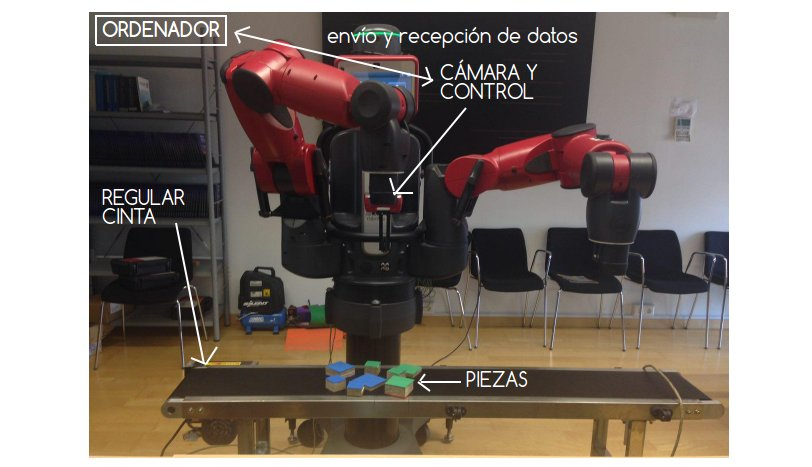
\includegraphics[scale=0.45]{imagenes/esquema.jpg}
	\caption{Esquema general del escenario.}
\end{figure}

\subsection{Visión por computador}
\noindent Como base para realizar la visión se ha utilizado un filtro de color \cite{maik}, a partir del cual se realiza la clasificación de objetos por color y posición. \\
\noindent En esta sección se explicarán estas funciones, que se pueden dividir en reconocimiento de objetos y procesamiento de imágenes. \\

\subsubsection{Reconocimiento de objetos}
\noindent Utilizando los tópicos de ROS se obtiene la imagen captada por la cámara del brazo derecho de Baxter, a partir de la cual se puede operar utilizando una función de \textit{callback} si existe, es decir, la función que se ejecutará al suscribirse al tópico de la cámara. En este caso esa función existe y se llama \textit{ImageCallback}. \\
\noindent Una vez se ha suscrito, es necesario conocer el color de los objetos rectangulares para reconocer su posición, tamaño y orientación, ya que sólo detectará los colores predefinidos en el código. Esto se realiza en formato HSV, estableciendo un rango para cada color de forma que estos se puedan filtrar en la imagen dejando el fondo negro; se han elegido colores con valores HSV lo bastante diferentes como para poder reconocerlos fácilmente, el azul y el verde. \\

\noindent Para calcular estos valores HSV, se ha utilizado el archivo hsvThresholder.py \cite{thpy}, al que se le pasa la imagen captada por la cámara de Baxter, que se puede ejecutar con el comando: \\

\textit{python hsvThresholder.py image.jpg} \\

\noindent Para obtener estos valores, es recomendable lanzar el programa para más imagenes con distintas posiciones de los objetos y distina iluminación. Se realizan capturas de los objetos con la máxima y la mínima iluminación posible, obteniendo un rango de valores HSV para los que se reconoce ese color. \\

\noindent Una vez se han reconocido los objetos que presentan los colores predefinidos, se obtiene su centro y se realiza un interlineado por sus bordes. En la siguiente figura \ref{fig:capter} se muestran distintas piezas identificadas en la ventana de visualización. Como se dijo anteriormente, estos objetos se han buscado por color en la captura proporcionada por el tópico de la cámara del brazo derecho. Se han obtenido sus centros en coordenadas de imagen, a partir de los cuales se han definido sus perímetros mediante líneas de color negro. \\

\begin{figure}[H]
	\centering % si queremos la imagen centrada
	\label{fig:capt}
	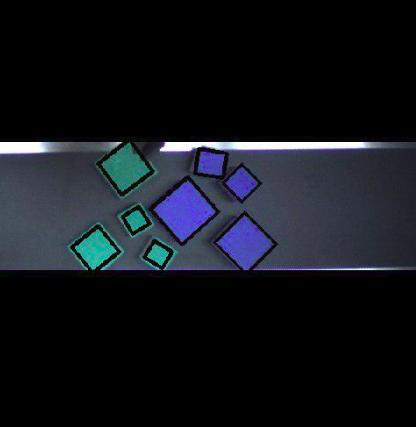
\includegraphics[scale=0.5]{imagenes/captura.jpg}
	\caption{Captura que muestra el reconocimiento de los objetos y la definición de sus perímetros.}
\end{figure}

\begin{figure}[H]
	\centering % si queremos la imagen centrada
	\label{fig:capter}
	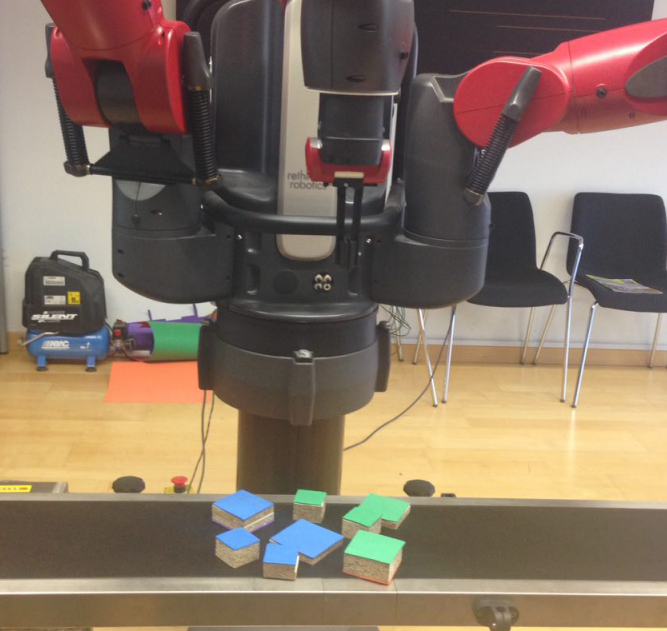
\includegraphics[scale=0.4]{imagenes/Baxter.png}
	\caption{Imagen que muestra la configuración de objetos de la imagen anterior \ref{fig:capt} desde fuera.}
\end{figure}

\subsubsection{Procesamiento de imágenes}
\noindent Al obtener la captura a través del tópico, se realiza una copia de esta a un tipo de dato correspondiente a una clase de OpenCV para imágenes, y se buscan, color por color, los objetos disponibles en esta imagen. \\

\noindent Para el posible ruido que pueda tener la imagen, se utiliza la función \textit{cvSmooth()} \cite{smooth} de OpenCV y se realiza un filtrado del rango de color que se está buscando en ese momento, dejando todo lo demás en negro. Se hace uso de la función \textit{cvErode()} \cite{erode} de OpenCV para borrar algunos puntitos blancos que pueden quedar tras filtrar la imagen. Tras esto, la imagen se pasa a escala de grises y se obtienen sólo los píxeles del objeto, logrando reconocer el rectángulo que lo define. El resultado de los objetos con el interlineado se muestra en una ventana de visualización (figura \ref{fig:capt}), por lo que el usuario puede determinar la calidad de detección de objetos con las características del entorno en el que se encuentra. \\

\noindent Una vez se ha conseguido obtener el centro de todos los objetos visibles en la imagen, se realiza el clustering con el algoritmo K-means (explicado en el anexo \ref{clustering}). Para ello, es imperativo el uso de un tipo de dato de OpenCV llamado \textit{Mat}, a través del que se copia un tipo de dato \textit{PoseArray}, un array de \textit{PoseStamped} que incluye las coordenadas de posición \textit{x, y, z} y las coordenadas de orientación, \textit{x, y, z, w}. Como se explicó en la sección de gestión de problemas (\ref{planif}), a través de este tipo de dato se le ha pasado tanto la posición del objeto como el color del mismo. \\
De la salida resultante del K-means se obtienen las etiquetas de cada uno de los objetos, siendo 0 si pertenece al clúster 0 y 1 si pertenece al 1, además de la posición obtenida en la última iteración de k-medias de los centroides que se han utilizado para obtener esos grupos, a partir de los que podemos calcular el punto medio y la orientación para realizar la clasificación. \\

\noindent Como todos estos cálculos se han realizado a partir de la imagen, las coordenadas que se han obtenido no nos valen para realizar las tareas de control, por ello, para enviar a través de un \textit{publisher} de ROS el valor del punto medio hay que realizar una conversión a coordenadas del mundo real, para lo que es necesario añadir desplazamientos, calculados empíricamente, a la conversión de las coordenadas \textit{x} e \textit{y} a coordenadas de la ``base'' de la escena de MoveIt!, ya que a la hora de realizar cualquier movimiento, este va a estar relacionado con la ``base'' en esta escena. \\

\subsection{Procedimientos de control}
\noindent Para la implementación de estas tareas se ha utilizado el lenguaje Python junto con el paquete \textit{moveit\_commander}, que permite realizar movimientos rectos con distinta orientación del \textit{gripper} o pinza. \\
\noindent Para realizar las tareas de clasificación, se han utilizado como herramientas una paleta y una cuña fabricadas a partir de cartón y goma eva, ya que las existentes, vistas en la sección \ref{chw}, no eran adecuadas para realizar este proyecto, puesto que se está trabajando con más de un objeto a la vez. \\

\subsubsection{\textit{Pick and place} adaptado}
\noindent Para este programa, se ha adaptado el código de \textit{pick and place} proporcionado por Gazebo. Gazebo \cite{gazebo} es un simulador de robots en 3D de código abierto que incluye una gran variedad de modelos y resulta bastante útil a la hora de realizar pruebas, diseñar o mejorar las implementaciones. Además permite crear un entorno acorde con el real y simular interacciones.\\
Esta implementación de la que se habla está destinada a ser ejecutada en este simulador. En este proyecto, como ejercicio de adaptación se ha utilizado este programa junto con visión por computador para realizar un \textit{pick and place} en el Baxter real (figura \ref{cd:pnp}).\\

\begin{figure}[H]
	\centering % si queremos la imagen centrada
	\label{cd:pnp}
	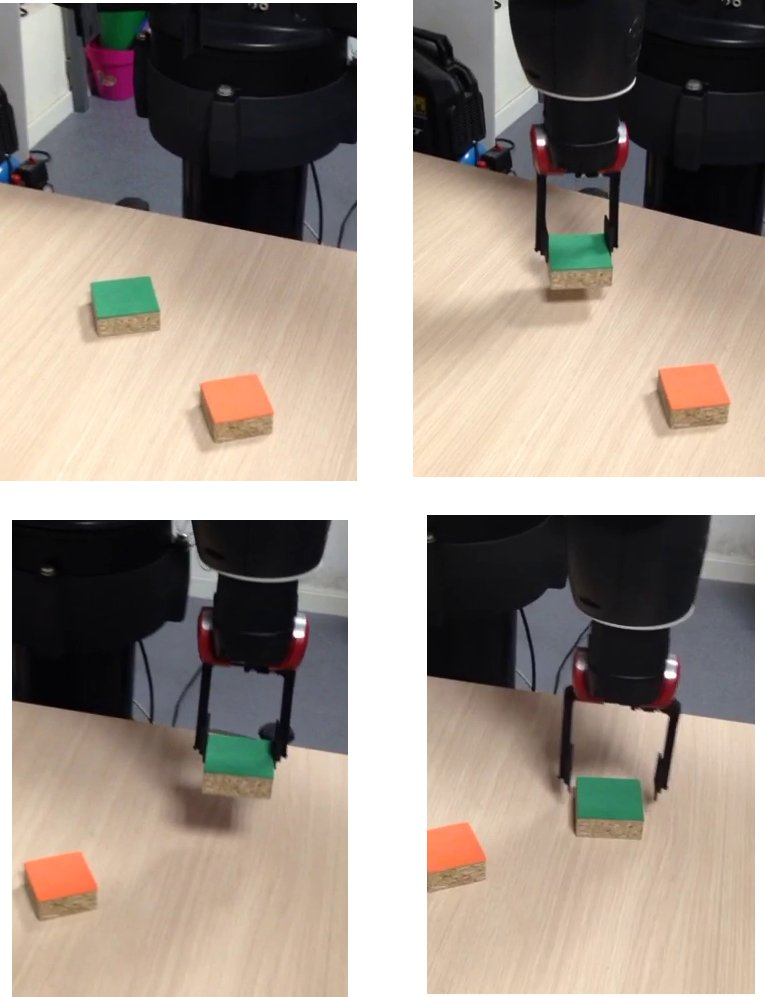
\includegraphics[scale=0.25]{imagenes/pandp.jpg}
	\caption{Capturas de la ejecución de \textit{pick and place} adaptado.}
\end{figure}

\subsubsection{Clasificación en entorno estático}
\noindent Conociendo el punto medio obtenido por el programa de visión, utilizando la paleta (figura \ref{cd:paleta}), Baxter mueve su brazo hasta esta posición con una orientación que también ha obtenido. Cuando se encuentra en esta posición, gira el \textit{gripper} hasta que forme 90º situándose en un eje horizontal y arrastra los objetos hacia arriba y hacia abajo, separándolos entre sí (figura \ref{cd:ce}). \\

\begin{figure}[H]
	\centering % si queremos la imagen centrada
	\label{cd:paleta}
	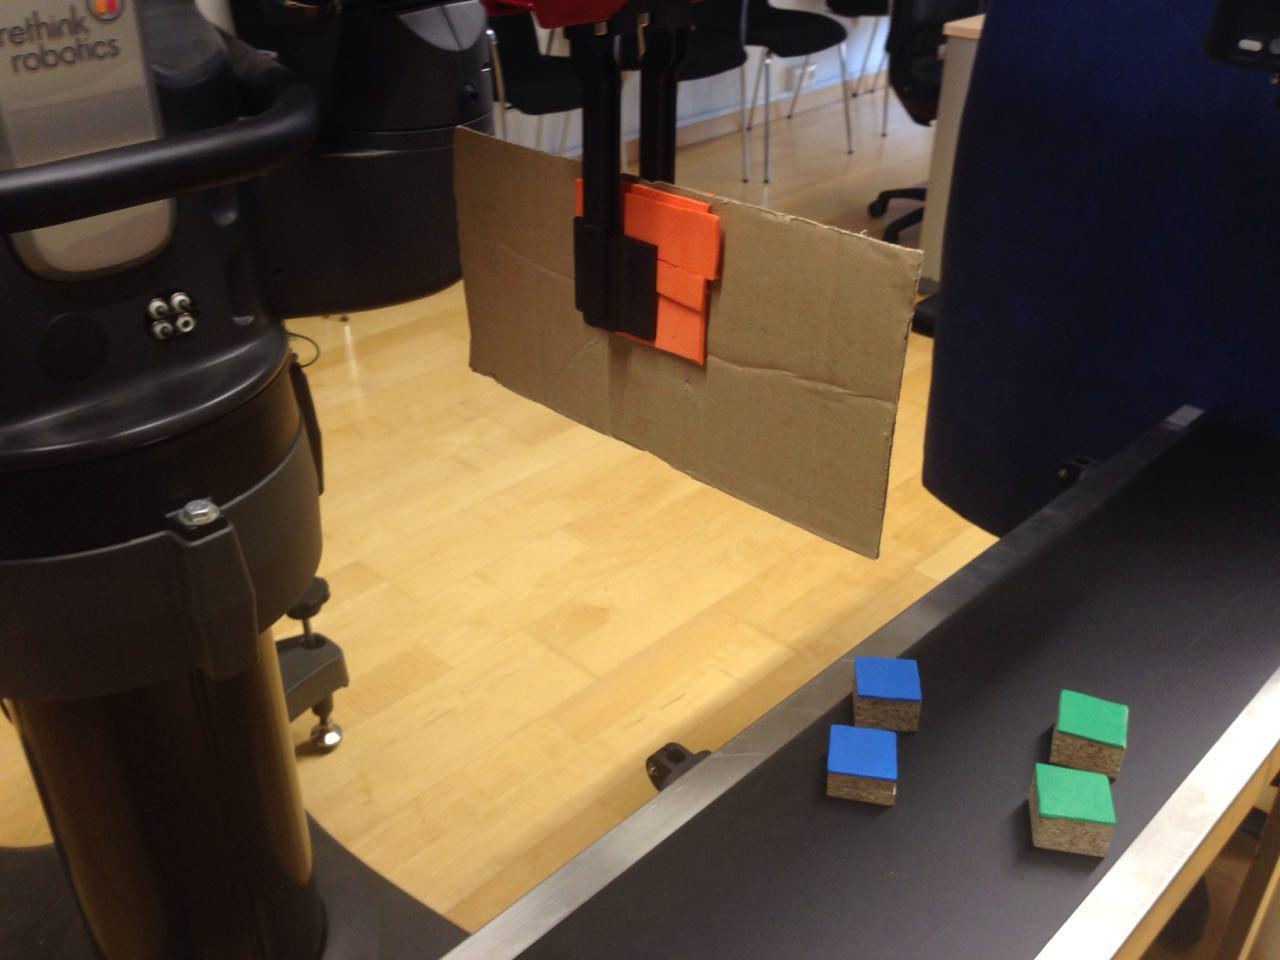
\includegraphics[scale=0.23]{imagenes/paleta.jpg}
	\caption{Paleta de cartón.}
\end{figure}

\begin{figure}[H]
	\centering % si queremos la imagen centrada
	\label{cd:ce}
	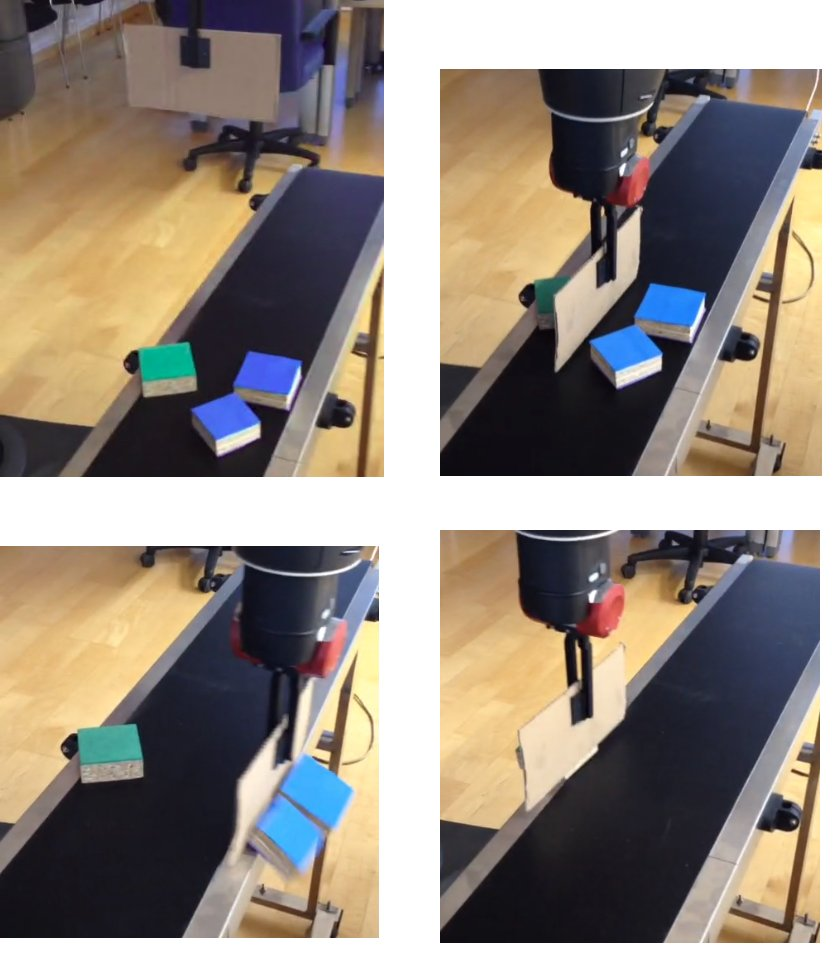
\includegraphics[scale=0.25]{imagenes/static.jpg}
	\caption{Capturas de la clasificación en entorno estático.}
\end{figure}

\subsubsection{Clasificación en entorno dinámico con cinta transportadora}
\noindent En este tipo de clasificación se han utilizado dos prototipos de herramienta, una cuña y una paleta hechas de cartón y goma eva para evitar el deslizamiento; sin embargo en una aplicación real, deberían utilizarse materiales más pesados y robustos, puesto que en ocasiones no se obtienen los resultados esperados debido al peso, rigidez o forma de estas sencillas herramientas construidas para la realización del proyecto. \\

\noindent El comienzo de ambas tareas es el mismo, obteniendo la posición en dos ocasiones separadas en el tiempo para conocer la velocidad y predecir en qué posición estarán en el momento de la separación. \\
\begin{enumerate}
	\item Clasificación utilizando como herramienta una paleta \ref{cd:paleta}\\
	
	Con esta herramienta se ha diseñado un comportamiento que separe primero los objetos de una clase y después los de la otra, calculando de nuevo la posición en la que se encontrarán entonces. \\ 
	Una vez conocemos la posición en la que estarán, el \textit{gripper} se sitúa en ese punto y espera a que los objetos lleguen, después separa en primer lugar los de abajo, apartándolos con la paleta en la dirección y con la orientación adecuadas. En ese momento además obtiene el punto en el que estarán situados los demás y al terminar de separar los anteriores va hacia esa posición, en la que realiza un movimiento análogo al realizado anteriormente pero en la dirección contraria (figura \ref{cd:pd}). \\
	
	\begin{figure}[H]
		\centering % si queremos la imagen centrada
		\label{cd:pd}
		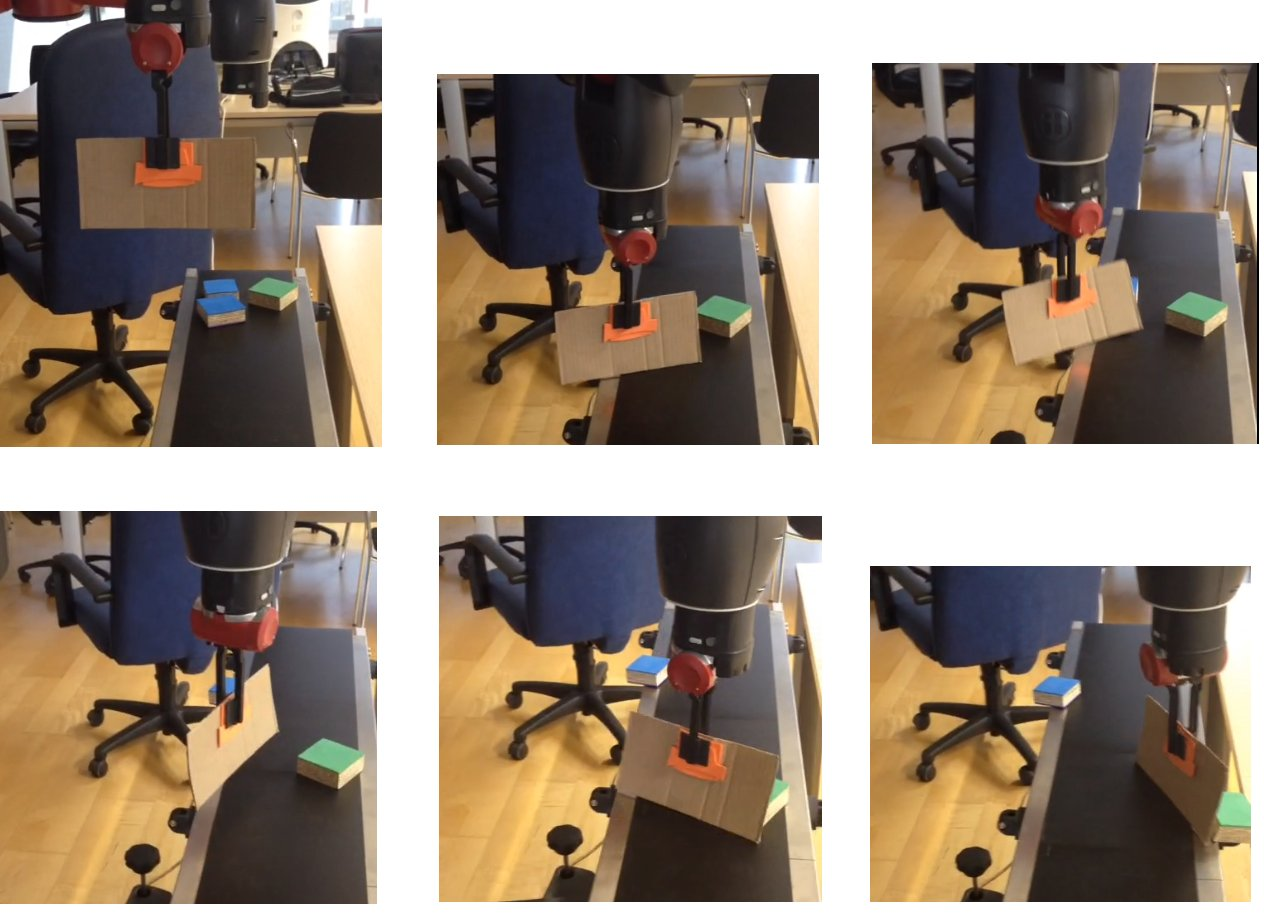
\includegraphics[scale=0.21]{imagenes/paletadyn.jpg}
		\caption{Capturas de la ejecución de la segmentación con paleta en entorno dinámico.}
	\end{figure}
	
	\item Clasificación utilizando como herramienta una cuña \\
	
	\begin{figure}[H]
		\centering % si queremos la imagen centrada
		\label{cd:cuna}
		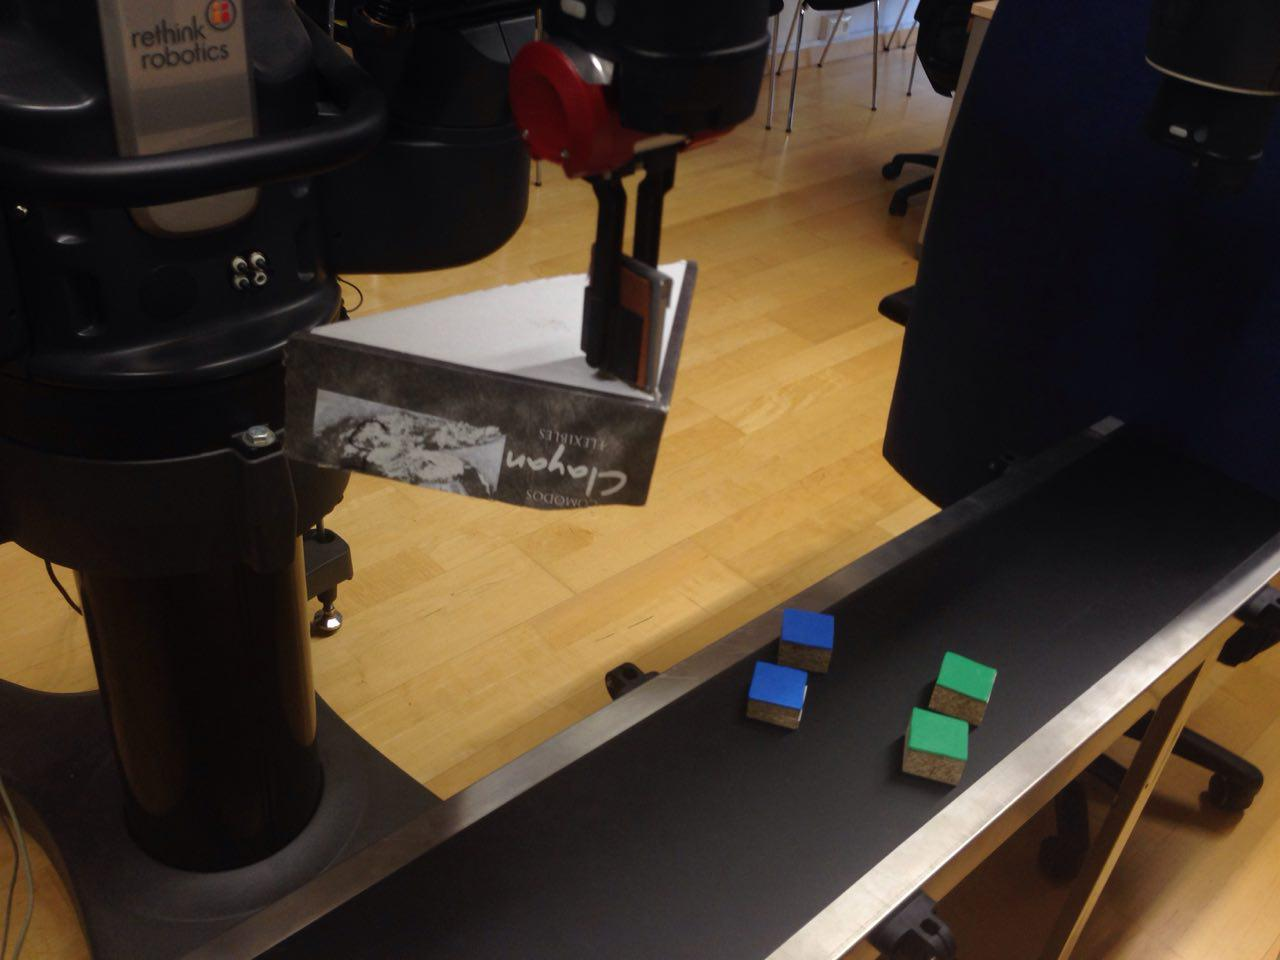
\includegraphics[scale=0.25]{imagenes/cunia.jpg}
		\caption{Cuña de cartón.}
	\end{figure}

	La cuña \ref{cd:cuna} es una herramienta que hace mucho más sencillo el control en este tipo de clasificación con cinta transportadora, por lo que las pruebas se realizarán con ella. Una vez se conoce la posición inicial, Baxter sitúa el brazo un poco más alejado de esta y con distinta orientación, de forma que pueda clasificar elementos cuya recta de separación tenga una pendiente más pronunciada. Cuando se detecta que los objetos han llegado a la posición en la que se encuentra la cuña, va hacia el punto que había calculado en un principio y avanza, de forma que los elementos se topen con los lados de la cuña y caigan fuera de la cinta transportadora, ayudándose de una oscilación en el eje vertical. (figura \ref{cd:cd})\\
	
	\begin{figure}[H]
		\centering % si queremos la imagen centrada
		\label{cd:cd}
		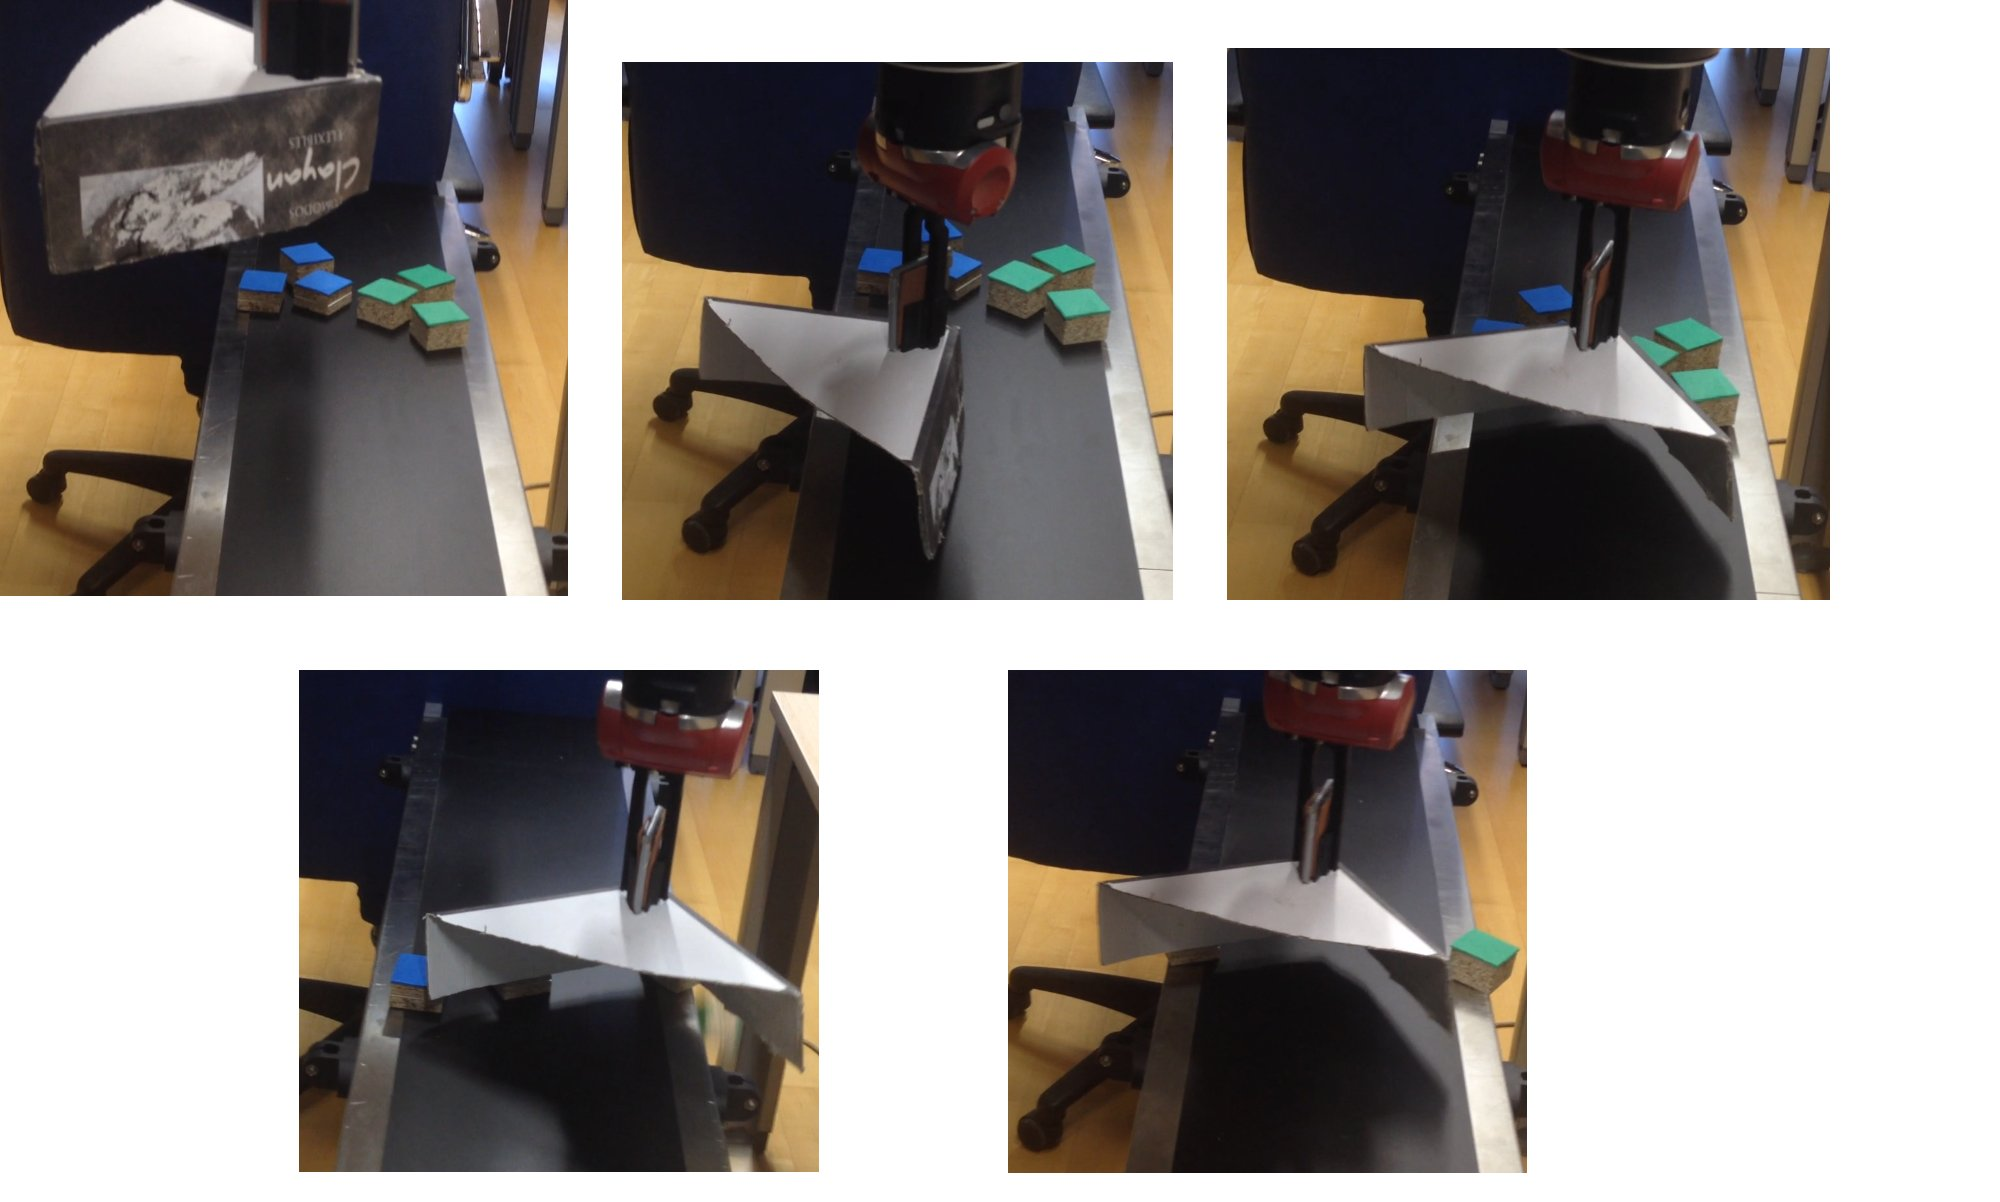
\includegraphics[scale=0.18]{imagenes/cunadyn.jpg}
		\caption{Capturas de la ejecución de la segmentación con cuña en entorno dinámico.}
	\end{figure}

\end{enumerate}